\documentclass{article}

% The file ijcai16.sty is the style file for IJCAI-16 (same as ijcai07.sty).
\usepackage{ijcai16}

% Packages
\usepackage{./std_package_reqs}

% Definitions
\usepackage{./definitions}

\usepackage{verbatim}

% Graphics Path
\graphicspath{{./images/}}

\renewcommand*{\mkbibparens}[1]{{\ifcitation{\bibleftbracket#1\bibrightbracket}%
        {\bibleftparen#1\bibrightparen}}}
\renewcommand*{\bibopenparen}[1]{{\ifcitation{\bibleftbracket#1}{\bibleftparen#1}}}
\renewcommand*{\bibcloseparen}{{\ifcitation{\bibrightbracket}{\bibrightparen}}}

% Bibliography
\addbibresource{references.bib}

\begin{document}
    
%--------------------------------------------------------------------------------------------------
% Front Matter
%--------------------------------------------------------------------------------------------------

    \title{Parameterized Hybrid Markov Decision Processes}

%\author{Shamin Kinathil \\
%ANU and NICTA \\
%Canberra, ACT, Australia \\
%shamin.kinathil@anu.edu.au \\
%\And
%Harold Soh \\
%\And
%Scott Sanner  \\
%NICTA and ANU \\
%Canberra, ACT, Australia \\
%ssanner@nicta.com.au \\
%}

\maketitle
    \begin{abstract}

Markov Decision Processes (MDPs) provide a powerful framework for
decision-theoretic planning.  While MDPs occur in many applications,
their applicability is limited by the common assumption that the model
parameters are known.  However, there are many settings where it is
important to solve or evaluate MDPs in the presence of uncertainty
over parameters, for example: (i) to investigate the trade-off between
different reward criteria in a multi-objective setting; (ii) to
perform sensitivity analyses of policies to various parameter
settings; and (iii) to analyse and optimise policy performance as a
function of policy parameters. However, formalizing MDPs in this way
leads to a family of hybrid (mixed discrete and continuous state and
action) MDPs with non-linear and/or piecewise structure. In this paper
we show how each of the aforementioned use cases can be formalized
under the common framework of parameterized hybrid MDPs and solved
exactly and in closed-form by leveraging techniques from symbolic
dynamic programming. Our novel framework allows one to explore for the
first-time: (i) an exact functional representation of the
multi-objective trade-offs for use in (Interactive) Decision Maps;
(ii) exact sensitivity analysis of public health policies in epidemic
models over the full range of infection rate parameters; and (iii)
non-convex optimization of policy parameters applied to finance
problems previously impossible with sample-based policy gradient
techniques.

\end{abstract}


%--------------------------------------------------------------------------------------------------
% Body
%--------------------------------------------------------------------------------------------------

    \section{Introduction}
\label{sec:introduction}

Markov Decision Processes (MDPs)~\parencite{Howard_MIT_1960} are the de facto standard framework for decision theoretic planning in fully
observable environments~\parencite{Boutilier_JAIR_1999}. MDPs occur in a wide range of real world domains such as game playing~\parencite{Szita_RL_2012}, power systems~\parencite{Reddy_IJCAI_2011}, ecology~\parencite{Williams_EM_2009} and patient admission
scheduling~\parencite{Zhu_AIM_2014}. Traditional MDP solution techniques often assume that the parameters of the model are
known. However, in practice, model parameters are usually estimated from limited data or elicited from humans and hence are naturally uncertain.  This often raises a critical in real world applications to (i) investigate the trade-off between different reward criteria in a multi-objective setting; (ii) perform sensitivity analyses of policies to various parameter settings; and (iii) analyse and optimise policy performance as a function of policy parameters.  Formalising models to address each of the aforementioned use cases is often fraught, due to the
specification leading to hybrid (mixed discrete and continuous state and/or action) MDPs with non-linear and/or piecewise structure that have been traditionally very difficult to solve.

In this paper we make the following key contributions:
\begin{itemize}
\item We present the unifying framework of {\it parameterized hybrid MDPs} (PHMDPs) which enables the investigation of trade-offs between
  multi-objective reward criteria, parameter sensitivity analysis and non-convex analysis and optimization of policy parameters
\item We provide an algorithm that solves this class of PHMDPs exactly and in closed-form by defining a Parameterized variant of Symbolic Dynamic Programming (SDP)~\parencite{Boutilier_IJCAI_2001} extended to hybrid MDPs~\parencite{Sanner_UAI_2011}
\item We use our novel framework to explore, for the first time: (i) an exact functional representation of the multi-objective
  trade-offs for use in interactive decision maps; (ii) exact sensitivity analysis of public health policies in epidemic models; and (iii) non-convex optimization of policy parameters applied to the optimal execution problem in finance
\end{itemize}
We remark that prior to this paper, it was an open question as to whether all of the above use cases admitted closed-form solutions --- these questions are resolved affirmatively through PHMDPs and SDP.

%This paper is organised as follows: In Section~\ref{sec:hybrid_mdps} we describe parameterized hybrid Markov Decision Processes (MDPs) and value iteration~\parencite{Bellman_PU_1957}, a widely used dynamic programming method for solving MDPs. Following this, in Section~\ref{sec:sdp}, we introduce Symbolic Dynamic Programming (SDP), and show how it can be used to calculate exact closed-form solutions to parameterized hybrid MDPs. In Section~\ref{sec:results} we calculate exact solutions to three empirical domains: (1) autonomous driving; (2) influenza epidemiology; and (3) optimal trade execution. We conclude in Section~\ref{sec:conclusion} and identify interesting directions for future research.

    \section{Related Work}
\label{sec:background}

%\begin{itemize}
%    \item MOMDPs - Pareto front methods (approximate), convex hull algorithm (exact) -- works for discrete parameterized MDPs, but not for factored or hybrid case -- we want to look at parameterized hybrid, no exact work in this space
%    \item Sensitivity analysis of MDPs -- but none exact in hybrid case
%    \item Policy gradient -- everything is numerically oriented, never a closed-form exact solution as a function of parameter, e.g., to analyze stability
%\end{itemize}

In this work, we present parameterized hybrid MDPs as a unifying framework which allows for multi-objective reasoning, exact
sensitivity analysis and parametric policy gradient analysis and optimisation.  While there are no comparable frameworks which allow
for the same breadth of functionality, we briefly survey prior art in each of these three areas and conclude with a discussion of alternate 
uses of the term \emph{parameterized} in the MDP literature that contrast with our contributions in this work.
%to establish the fundamental importance of each of these problems.

The Multi-objective MDP (MOMDP) literature studies the solution and analysis of trade-offs in the presence of multiple reward criteria.
The techniques used to solve MOMDPs with unknown preferences depend on the nature of the scalarization function used to weight each reward
component~\parencite{Roijers_JAIR_2013}. If the scalarization function is linear, then methods such as the Convex Hull Value Iteration
algorithm~\parencite{Barrett_ICML_2008}, which returns the optimal policy for discrete \emph{enumerated state} MOMDPs with any linear
preference function, can be used. For non-linear scalarization functions the Pareto front of a set of undominated policies must be
returned. The Pareto front can be prohibitively large and as a result solution techniques such as those of~\parencite{Chatterjee_STACS_2006}
and~\parencite{Pirotta_AAAI_2015} have focussed on approximating the Pareto front, or using a refinement of Pareto dominance known as
Lorenz optimality~\parencite{Perny_AAAI_2013} to further restrict the size of the solution set.  User-oriented tools like (Interactive)
Decision Maps~\parencite{Lotov_IDM} allow one to visualise and analyse the reward trade-offs associated with all parameter settings.  In this work we present \textit{exact} \emph{factored hybrid} MOMDP solutions via the framework of PHMDPs and SDP.
%multi-objective closed-form solutions to the more general class of
%\textit{parameterized hybrid} MDPs with factored states.

Sensitivity analysis of MDP parameters is a critical tool in understanding what parameters are most important to measure well and how MDP policies vary over a range of parameters.  To date, most work has focussed on uncertainty within the specification the transition function~\parencite{Kalyanasundaram_AJC_2004}, reward function~\parencite{Tan_JAP_2011, Hopp_JOTA_1988}, or a combination of both~\parencite{Givan_AI_2000}, in discrete MDPs. The framework that we introduce in this paper enables \textit{exact} sensitivity analysis
for PHMDPs that allows it to be applied in continuous state settings and permits the derivation and analysis of the \emph{optimal} policy as a
function of these parameters.

Policy gradient methods rely upon optimizing parameterized policies with respect to the expected return by gradient descent. The main
concern of such methods is obtaining a good estimator of the policy gradient~\parencite{Peters_IRS_2006}. Two of the most prominent
approaches have been the finite-difference methods such as those of~\parencite{Ng_UAI_2000} and Monte Carlo methods such as~\parencite{Sutton_NIPS_1999,Baxter_ISCAS_2000}, both of which are numerically oriented and sample based. Our use of PHMDPs and SDP allows for us to solve for an \emph{exact} policy value as a parameterized function of policy parameters, hence permitting exact gradient analysis as well as the direct application of (non-)convex optimization to this parameteric value form.
% Have to cite Sutton!  If anything, drop Baxter but try not to.
% Also ``non-convex functions of parameters'', not ``non-convex parameters''

Finally, as a point of differentiation from other uses of the term \emph{parameterized} in the MDP literature, we remark that other works~\parencite{Duff_UMA_2002,Dearden_UAI_1999,Gopalan_COLT_2015} have used Parameterized MDP to refer to MDPs with latent parameters whose
beliefs can be updated by observing reward and transition samples. In contrast, in this work we assume strict uncertainty of continuous MDP
parameters in models that are otherwise fully specified; in this way we can treat parameters simply as free variables that can be parametrically analysed via recent advances in symbolic solution methods.



    \section{Parameterized Hybrid MDPs}
\label{sec:hybrid_mdps}

In this section we introduce parameterized hybrid Markov Decision
Processes (PHMDPs) and show how the framework can be specialized to
address multi-objective reward criteria, investigate parameter
sensitivity and optimize continuous non-convex policy parameters. We
also review their finite horizon solution via dynamic programming.

\subsection{Definition}
\label{sec:hybrid_mdps_def}

A parameterized hybrid Markov Decision Process (PHMDP) is defined by the tuple {\footnotesize \PMDPTuple}. {\footnotesize \State} specifies
a vector of states given by {\footnotesize $(\vec{d}, \vec{x}) =  \left( d_1, \ldots, d_m, x_1, \ldots, x_n \right) $}, where each {\footnotesize $ d_i \in \left\lbrace 0, 1 \right\rbrace $} {\footnotesize $\left( 1 \leq i \leq m \right)$} is discrete and each
{\footnotesize$ x_j \in \Real $} {\footnotesize $\left( 1 \leq j \leq   n \right)$} is continuous. {\footnotesize \Action} specifies a
finite set of actions.  {\footnotesize $\vec{\theta} \in \Theta$} are free parameters from the parameter space {\footnotesize $ \Theta $}. PHMDPs are naturally factored~\parencite{Boutilier_JAIR_1999} in terms of the state variables {\footnotesize$\vec{d}$} and {\footnotesize
$\vec{x}$}. Hence, the joint transition model can be written as:
{\footnotesize
\abovedisplayskip=0pt
\belowdisplayskip=0pt
\begin{align}
    \label{eq:hmdp_tfunc}
    \Transition :& \, \ProbArg{\vec{d}', \vec{x}' | \vec{d}, \vec{x}, a, \vec{\theta}} = \nonumber \\
    & \prod_{i=1}^{m} \ProbArg{d_i' | \vec{d}, \vec{x}, a, \vec{\theta}} \prod_{j=1}^{n} \ProbArg{x_j' | \vec{d}, \vec{d}', \vec{x}, a, \vec{\theta}}.
\end{align}   
}

{\footnotesize \RewardFunc} is the reward function which encodes the preferences of the agent. {\footnotesize \Horizon} represents the
number of decision steps until termination and the discount factor {\footnotesize $\gamma \in [0, 1)$} is used to geometrically discount
future rewards.

A policy {\footnotesize $\pi : \State \rightarrow \Action$}, specifies
the action to take in every state. The value of a state {\footnotesize
  $(\vec{d}, \vec{x}) \in \State$} under a given policy
{\footnotesize$\pi$} is given by: {\footnotesize
    \abovedisplayskip=0pt
    \belowdisplayskip=0pt
\begin{align*}
    V^{\pi}\left( \vec{d}, \vec{x}; \vec{\theta} \right) &= \Exp{\sum\limits_{h = 0}^{\Horizon} \gamma^h \cdot r^h | \vec{d}, \vec{x}, \vec{\theta}} \nonumber  
%    &= \sum\limits_{s' \in \State}  \Transition\left(s, \pi\left(s\right), s' \right) \left[ \Reward\left(s, \pi(s), s'\right) + \gamma \cdot V^{\pi}(s')\right]. \label{eq:mdp_bellman_eq}
\end{align*}
}
%Equation~\eqref{eq:mdp_bellman_eq} is known as the Bellman equation for $V^{\pi}$.

The state-action value function {\footnotesize$Q : \State \times \Action \rightarrow \mathbb{R}$} is given by:
{\footnotesize 
    \abovedisplayskip=0pt
    \belowdisplayskip=0pt
\begin{align}
    \label{eq:mdp_qfunc}
    Q^{\pi}\left(\vec{d}, \vec{x}, a; \vec{\theta}\right) = \Exp{\sum\limits_{h = 0}^{\Horizon} \gamma^h \cdot r^h | \vec{d}, \vec{x}, a, \vec{\theta}}. 
\end{align}
}

The value function of the optimal policy {\footnotesize$ \pi^{*} $} satisfies:

{\footnotesize 
\abovedisplayskip=0pt
\belowdisplayskip=0pt
\begin{align}
    \label{eq:opt_vfunc}
    V^{\pi^{*}}(\vec{d}, \vec{x}; \vec{\theta}) &= \max_{a \in A} \left\{ Q^{\pi^{*}}(\vec{d}, \vec{x}, a; \vec{\theta}) \right\}. 
\end{align}
}%

We again remark that in our formulation of PHMDPs the
parameters {\footnotesize $ \vec{\theta} $} are free parameters and not
learned from reward and transition samples as discussed in Related Work.
We also remark that we are not assuming a (Bayesian) reinforcement learning setting,
but rather a setting of strict uncertainty over {\footnotesize $ \vec{\theta} $} and
a parameterized symbolic value iteration solution to solve it.

In the subsequent sections we demonstrate how the PHMDP framework can
be specialised into models capable of: (i) investigating
multi-objective reward criteria; (ii) exact parameter sensitivity
analysis; and (iii) optimization of continuous non-convex policy
parameters.

\subsubsection{Multi-objective PHMDPs}

The PHMDP framework can be specialised into a multi-objective setting
by specifying the reward as {\footnotesize \MORewardFunc} where
{\footnotesize $ d $} is the dimension of the reward vector. In this
formulation the parameter {\footnotesize $ \vec{\theta}^{d} $} specifies the
linear scalarization over the reward components (i.e, {\footnotesize $\langle
\Reward, \vec{\theta}^{d} \rangle$}) and the value function can be expressed
as a function of all possible scalarizations.

\subsubsection{Sensitivity Analysis for PHMDPs}

In sensitivity analysis, we assume that {\footnotesize $\vec{\theta}^{d}$} are unknown
parameters and we solve directly for the value function in
Equation~\eqref{eq:opt_vfunc} as a parametric function
{\footnotesize $V^{\pi^{*}}(\vec{d}, \vec{x}; \vec{\theta}^{d})$} of these parameters.  This
parametric value function can then be directly analyzed or displayed in an
(Interactive) Decision Map, an example of which is shown in
section~\ref{sec:results_influenza}, which allows a user to explore
trade-offs between parameters {\footnotesize $\vec{\theta}^{d}$ }for the optimal policy as a
function of other state variables {\footnotesize $\vec{d},\vec{x}$}.

\subsubsection{Policy Gradient Methods for PHMDPs}

PHMDP policy parameters can be analyzed and optimised by parameterizing a policy {\footnotesize $\pi$} by action parameters {\footnotesize $\vec{\theta}^{d}$}, and evaluating the value w.r.t. this parametric policy, an example of which will be shown in section~\ref{sec:results_oe}. The resulting (non-convex) policy value as a function of {\footnotesize $\vec{\theta}^{d}$} can be
analyzed, and optimised using the parameteric form of {\footnotesize $V^{\pi^{*}}(\vec{d}, \vec{x}; \vec{\theta}^{d})$} and all symbolic
derivatives (up to any order) of this value function.

\subsection{Solution Methods}

Value iteration~\parencite{Bellman_PU_1957} is a general dynamic
programming algorithm used to solve MDPs. We modify the algorithm to
solve the parameterized hybrid MDP formulation presented in
section~\ref{sec:hybrid_mdps_def}. The key idea of VI is to
successively approximate {\footnotesize $V^{\pi^{*}}(\vec{d}, \vec{x};
  \vec{\theta})$} and {\footnotesize $Q^{\pi^{*}}(\vec{d}, \vec{x}, a;
  \vec{\theta})$} by {\footnotesize $V^{h}(\vec{d}, \vec{x}; \vec{\theta})$} and
{\footnotesize $Q^{h}(\vec{d}, \vec{x}, a; \vec{\theta})$}, respectively, at
each horizon {\footnotesize$h$}. These two functions satisfy the
following recursive relationship:

{\footnotesize 
    \abovedisplayskip=0pt
    \belowdisplayskip=0pt
    \begin{align}
        Q^{h}(\vec{d}, \vec{x}, a; \vec{\theta}) = \Reward(\vec{d}, \vec{x}, a; \vec{\theta}) + \gamma \, \cdot &  \nonumber \\ 
        \sum_{\vec{d}'} \int_{\vec{x}'} \ProbArg{\vec{d}', \vec{x}' | \vec{d}, \vec{x}, a; \vec{\theta}} & \cdot V^{h-1}(\vec{d}, \vec{x}; \vec{\theta}) \, d\vec{x}'  \label{eq:vi_qfunc} \\
        V^{h}(\vec{d}, \vec{x}; \vec{\theta}) = \max_{a \in A} \left\{ Q^{h}(\vec{d}, \vec{x}, a; \vec{\theta}) \right\} & \label{eq:vi_vfunc}
    \end{align}
}%

{\footnotesize $\ProbArg{\vec{d}', \vec{x}' | \vec{d}, \vec{x}, a;
    \vec{\theta}}$ } is specified in Equation~\eqref{eq:hmdp_tfunc}. The
algorithm can be executed by first initialising {\footnotesize
  $V^{0}(\vec{d}, \vec{x}; \vec{\theta})$} to zero or the terminal
reward. Then for each {\footnotesize$h$}, {\footnotesize
  $V^{h}(\vec{d}, \vec{x}; \vec{\theta})$} is calculated from {\footnotesize
  $V^{h-1}(\vec{d}, \vec{x}; \vec{\theta})$} via
Equations~\eqref{eq:vi_qfunc} and~\eqref{eq:vi_vfunc}, until the
intended $h$-stage-to-go value function is computed.

A key challenge still remains, namely, dealing with infinitely many
states in {\footnotesize $\vec{x}$} and {\footnotesize
  $\vec{\theta}$}. Furthermore, we must determine restrictions on
{\footnotesize $Q^{h}(\vec{d}, \vec{x}, a; \vec{\theta})$} and
{\footnotesize $V^{h}(\vec{d}, \vec{x}; \vec{\theta})$} that guarantee
tractable solutions. In the next section we show that a parameterized
extension of symbolic dynamic programming can be used to address these
concerns and optimally solve exactly and in closed-form PHMDPs for
arbitrary horizons.

    \section{Parameterized Symbolic Dynamic Programming}
\label{sec:sdp}

Symbolic Dynamic Programming (SDP)~\parencite{Boutilier_IJCAI_2001} is the process of performing dynamic programming via symbolic manipulation. In the following sections we present a brief overview of SDP operations and also show how SDP can be used to solve parameterized Hybrid MDPs.

\subsection{Symbolic Case Calculus}

SDP assumes that all functions can be represented in case statement form \parencite{Boutilier_IJCAI_2001} as follows:
{\footnotesize 
    \abovedisplayskip=5pt
    \belowdisplayskip=0pt
    \begin{align*}
        f = 
        \begin{cases}
            \phi_1: & f_1 \\ 
            \vdots & \vdots\\ 
            \phi_k: & f_k \\ 
        \end{cases}
    \end{align*}
}%

Here, {\footnotesize$ f_i $} are linear expressions over {\footnotesize$ \vec{x} $} and {\footnotesize$\phi_i$} are logical formulae defined over the state {\footnotesize$( \vec{d}, \vec{x})$} that can consist of arbitrary logical combinations of boolean variables and linear inequalities {\footnotesize$\left( \geq, >, <, \leq \right)$} over continuous variables. We assume that the set of conditions {\footnotesize$\left\lbrace \phi_1, \ldots, \phi_k \right\rbrace$} disjointly and exhaustively partition {\footnotesize$(\vec{d}, \vec{x})$} such that {\footnotesize$f$} is well-defined for all {\footnotesize$(\vec{d}, \vec{x})$}. In this paper we restrict the {\footnotesize$f_i$} to be either constant or linear functions of the state variable {\footnotesize$\vec{x}$}. Henceforth, we refer to functions with linear {\footnotesize$\phi_i$} and piecewise constant {\footnotesize$f_i$} as linear piecewise constant (LPWC) and functions with linear {\footnotesize$\phi_i$} and piecewise linear {\footnotesize$f_i$} as linear piecewise linear (LPWL) functions.

Operations on case statements may be either unary or binary. All of the operations presented here are closed form for LPWC and LPWL functions. We refer the reader to~\parencite{Sanner_UAI_2011,Zamani_AAAI_2012} for more thorough expositions of SDP for piecewise continuous functions.

Unary operations on a single case statement \emph{f}, such as scalar multiplication {\footnotesize$c \cdot f$} where {\footnotesize$ c \in \mathbb{R} $}, are applied to  each {\footnotesize$f_i \left(1 \leq i \leq k\right)$}. Binary operations such as addition, subtraction and multiplication are executed in two stages. Firstly, the cross-product of the logical partitions of each case statement is taken, producing paired partitions. Finally, the binary operation is applied to the resulting paired partitions. The ``cross-sum'' {\footnotesize$\oplus$} operation can be performed on two cases in the following manner:
{\footnotesize 
%    \abovedisplayskip=5pt
%    \belowdisplayskip=0pt
    \begin{center}
        \begin{tabular}{r c c c l}
            $\begin{cases}
            \phi_1: \hspace{-1mm} & \hspace{-1mm} f_1  \\ 
            \phi_2: \hspace{-1mm} & \hspace{-1mm} f_2  \\ 
            \end{cases}$
            $\oplus$
            &
            \hspace{-4mm}
            $\begin{cases}
            \psi_1: \hspace{-1mm} & \hspace{-1mm} g_1  \\ 
            \psi_2: \hspace{-1mm} & \hspace{-1mm} g_2  \\ 
            \end{cases}$
            &
            \hspace{-4mm} 
            $ = $
            &
            \hspace{-4mm}
            $\begin{cases}
            \phi_1 \wedge \psi_1: & f_1 + g_1 \\
            \phi_1 \wedge \psi_2: & f_1 + g_2 \\
            \phi_2 \wedge \psi_1: & f_2 + g_1 \\
            \phi_2 \wedge \psi_2: & f_2 + g_2  \\
            \end{cases}$
        \end{tabular}
    \end{center}
}%
%\vspace{-4em}

``cross-subtraction'' {\footnotesize$\ominus$} and ``cross-multiplication'' {\footnotesize$\otimes$} are defined in a similar manner but with the addition operator replaced by the subtraction and multiplication operators, respectively. Some partitions resulting from case operators may be inconsistent and are thus removed.

Substitution into case statements is performed via a set {\footnotesize$\vartheta$} of variables and their substitutions e.g. {\footnotesize$\vartheta = \left\{ x'_1/(x_1 + x_2) \right\}$}, where the LHS of the / represents the substitution variable and the RHS of the / represents the expression that should be substituted in its place. {\footnotesize$\vartheta$} can be applied to both non-case functions {\footnotesize$f_i$} and case partitions {\footnotesize$\phi_i$} as {\footnotesize$f_i\vartheta$} and {\footnotesize$\phi_i\vartheta$}, respectively. Substitution into case statements can be written as:
{\footnotesize 
    \abovedisplayskip=5pt
    \belowdisplayskip=0pt
    \begin{align*}
        f\vartheta = 
        \begin{cases}
            \phi_1\vartheta: & f_1\vartheta \\ 
            \vdots & \vdots\\ 
            \phi_k\vartheta: & f_k\vartheta \\ 
        \end{cases}
    \end{align*}
}%

Substitution is used when calculating integrals with respect to deterministic {\footnotesize$\delta$} transitions~\parencite{Sanner_UAI_2011}.

Maximisation over cases, known as $\casemax$, is defined as:
\vspace{-0.5em}
{\footnotesize 
    \abovedisplayskip=0pt
    \belowdisplayskip=0pt
    \begin{center}
        \begin{tabular}{r c c c l}
            \hspace{-7mm} 
            
            $\casemax \Bigg(
            \begin{cases}
            \phi_1: \hspace{-1mm} & \hspace{-1mm} f_1 \\ 
            \phi_2: \hspace{-1mm} & \hspace{-1mm} f_2 \\ 
            \end{cases}$
            $,$
            &
            \hspace{-4mm}
            $\begin{cases}
            \psi_1: \hspace{-1mm} & \hspace{-1mm} g_1 \\ 
            \psi_2: \hspace{-1mm} & \hspace{-1mm} g_2 \\ 
            \end{cases} \Bigg)$
            &
            \hspace{-4mm} 
            $ = $
            &
            \hspace{-4mm}
            $\begin{cases}
            \phi_1 \wedge \psi_1 \wedge f_1 > g_1    : & \hspace{-2mm} f_1 \\ 
            \phi_1 \wedge \psi_1 \wedge f_1 \leq g_1 : & \hspace{-2mm} g_1 \\ 
            \phi_1 \wedge \psi_2 \wedge f_1 > g_2    : & \hspace{-2mm} f_1 \\ 
            \phi_1 \wedge \psi_2 \wedge f_1 \leq g_2 : & \hspace{-2mm} g_2 \\ 
            \vdots & \vdots
            \end{cases}$
        \end{tabular}
    \end{center}
}%

$\casemax$ preserves the linearity of the constraints and the constant or linear nature of the {\footnotesize$f_i$} and {\footnotesize$g_i$}. If the {\footnotesize$f_i$} or {\footnotesize$g_i$} are quadratic then the expressions {\footnotesize$f_i > g_i$} or {\footnotesize$f_i \leq g_i$} will be at most univariate quadratic and any such constraint can be linearised into a combination of at most two linear inequalities by completing the square. 

A case statement can be maximised with respect to a continuous parameter {\footnotesize$y$} as {\footnotesize $ f_1(\vec{x}, y) = \contmax_{y}f_2(\vec{x}, y) $}. The continuous maximisation operation is a complex case operation whose explanation is beyond the scope of this paper. We refer the reader to~\parencite{Zamani_AAAI_2012} for further details.

In principle, case statements can be used to represent all PHMDP components. In practice, case statements are implemented using a more compact representation known as Extended Algebraic Decision Diagrams (XADDs)~\parencite{Sanner_UAI_2011}, which also support efficient versions of all of the aforementioned operations.

\subsection{SDP for Parameterized Hybrid MDPs}

To calculate the exact solution to PHMDPs we begin by replacing all functions and operations in Equations~\eqref{eq:vi_qfunc} and~\eqref{eq:vi_vfunc} by their case statement equivalents. That is, we exchange operations such as {\footnotesize$+$}, {\footnotesize$\times$} and {\footnotesize$\max$}, by their symbolic equivalents, {\footnotesize$\oplus$}, {\footnotesize$\otimes$} and $\casemax$, respectively, and express {\footnotesize $\Reward(\vec{d}, \vec{x}, a; \vec{\theta})$},  {\footnotesize $\ProbArg{\vec{d}', \vec{x}' | \vec{d}, \vec{x}, a, \vec{\theta}}$}, {\footnotesize $V^0(\vec{d}, \vec{x}; \vec{\theta})$} as case statements. The optimal solution to PHMDPs can now be described by the following recursive SDP equations:

{\footnotesize 
    \abovedisplayskip=0pt
    \belowdisplayskip=0pt
    \begin{align}
        Q^{h}(\vec{d}, \vec{x}, a; \vec{\theta}) = \Reward(\vec{d}, \vec{x}, a; \vec{\theta}) \oplus \gamma \, \cdot &  \nonumber \\ 
        \sum_{\vec{d}'} \int_{\vec{x}'} \ProbArg{\vec{d}', \vec{x}' | \vec{d}, \vec{x}, a; \vec{\theta}} & \otimes V^{h-1}(\vec{d}, \vec{x}; \vec{\theta}) \, d\vec{x}'  \label{eq:vi_sdp_qfunc} \\
        V^{h}(\vec{d}, \vec{x}; \vec{\theta}) = \casemax_{a \in A} & \left\{ Q^{h}(\vec{d}, \vec{x}, a; \vec{\theta}) \right\} \label{eq:vi_sdp_vfunc}
    \end{align}
}%

{\footnotesize $\ProbArg{\vec{d}', \vec{x}' | \vec{d}, \vec{x}, a; \vec{\theta}}$ } is specified in Equation~\eqref{eq:hmdp_tfunc}. We note that the parameters {\footnotesize $\vec{\theta}$} remain free variables during the backup operation, they are not regressed as are the continuous state parameters {\footnotesize $ \vec{x} $}. All operations including action maximization will automatically condition the value on these parameters, yielding the parameterized value function in Equation~\eqref{eq:vi_sdp_vfunc}.

In the case of discrete {\footnotesize \Action} it can be proved that all of the SDP operations used in Equations~\eqref{eq:vi_sdp_qfunc} and~\eqref{eq:vi_sdp_vfunc} are closed form for non-linear piecewise non-linear (NPWN) functions~\parencite{Sanner_UAI_2011}. In the case of continuous {\footnotesize \Action} all of the operations are closed form for only LPWC or LPWL functions~\parencite{Zamani_AAAI_2012}.

%It can be proved that all of the SDP operations used in Equations~\eqref{eq:vi_qfunc} and~\eqref{eq:vi_vfunc} are closed form for LPWC or LPWL functions~\parencite{Sanner_UAI_2011,Zamani_AAAI_2012}. Given a LPWL {\footnotesize $V^{0}(\vec{d}, \vec{x}; \vec{\theta})$} and that SDP operations are closed form, the resulting {\footnotesize $V^{1}(\vec{d}, \vec{x}; \vec{\theta})$} is also LPWL. Therefore, by induction is {\footnotesize $V^{h+1}(\vec{d}, \vec{x}; \vec{\theta})$} LPWL for all horizons {\footnotesize $ \Horizon $}. 

\subsubsection{Multi-objective PHMDPs}

PHMDPs with multi-objective {\footnotesize $\Reward$} and linear scalarization functions can be solved exactly and in closed-form by restricting the {\footnotesize $\Reward$} to LPWC functions and {\footnotesize $\Transition$} to LPWL functions. Given a LPWL {\footnotesize $V^{0}(\vec{d}, \vec{x}; \vec{\theta})$} and that SDP operations are closed form, the resulting {\footnotesize $V^{1}(\vec{d}, \vec{x}; \vec{\theta})$} is also LPWL. Therefore, by induction is {\footnotesize $V^{h+1}(\vec{d}, \vec{x}; \vec{\theta})$} LPWL for all horizons {\footnotesize $ h \in \Horizon $}.

Multi-objective PHMDPs with a non-linear scalarization function and NPWN {\footnotesize $\Reward$} and {\footnotesize $\Transition$} functions lead NPWN solutions which are exact, but not closed-form\parencite{Sanner_UAI_2011}.

\subsubsection{Sensitivity Analysis for PHMDPs}

%Sensitivity analysis for PHMDPs can be conducted exactly and in closed-form by firstly imposing the same restrictions on the {\footnotesize $\Reward$} and {\footnotesize $\Transition$} as the previous section and then differentiating the resulting value function with respect to the parameter {\footnotesize $\vec{\theta}$} i.e. {\footnotesize $\bigtriangledown_{\vec{\theta}} V^{h}\left(\vec{d}, \vec{x}; \vec{\theta}\right)$ }.

Sensitivity analysis for PHMDPs can be analysed exactly and in closed-form via SDP by first calculating Equation~\eqref{eq:vi_sdp_vfunc} and then taking symbolic derivatives, up to any order, with respect to the parameter {\footnotesize $\vec{\theta}$} i.e. {\footnotesize $\bigtriangledown_{\vec{\theta}} V^{h}\left(\vec{d}, \vec{x}; \vec{\theta}\right)$}.

\subsubsection{Policy Gradient Methods for PHMDPs}

Policy parameters for PHMDPs can be analysed exactly and in closed-form via SDP by calculating Equation~\eqref{eq:vi_sdp_qfunc} and \textit{not} Equation~\eqref{eq:vi_sdp_vfunc}. This is due to their being only one policy, which leads to one {\footnotesize $ Q^{h}(\vec{d}, \vec{x}, a; \vec{\theta}) $}. Because this function is parametric, it is possible to take symbolic derivatives up to any order i.e. {\footnotesize $\bigtriangledown_{\vec{\theta}} Q^{h}(\vec{d}, \vec{x}, a; \vec{\theta})$ } and apply non-convex optimization tools, such as polynomial programming~\parencite{sherali1992global}, that exploit parametric knowledge of the function.

In the next section we demonstrate how SDP can be used to compute exact solutions to a variety of parameterized hybrid MDPs.
    \section{Results}
\label{sec:results}

In this section we demonstrate the utility of our novel framework on three hitherto uninvestigated questions: (i) an exact functional representation of the multi-objective trade-offs in a multi-objective navigation domain; (ii) exact sensitivity analysis of public health policies in epidemic models over the full range of infection rate parameters; and (iii) non-convex optimization of policy parameters applied to finance problems previously impossible with sample-based policy gradient techniques.

\subsection{Multi-objective Navigation}
\label{sec:results_navigation}

In this domain we consider an autonomous vehicle moving along one dimension, e.g. along the real number line. At each stage the vehicle must trade-off between moving into a potentially higher reward region demarcated by a {\footnotesize $ \mathtt{threshold} $} and incurring a cost associated with movement. The domain is specified as follows:
\begin{itemize}
    \item {\footnotesize $ \State = \left\langle loc \right\rangle$}, where $ loc $ is the location of the vehicle
    \item {\footnotesize $ \Action \in \left\lbrace -5.0, 0.0, 5.0 \right\rbrace $} is the amount by which vehicle moves relative to its current location
    \item {\footnotesize $ \Transition\left( loc' | loc, a \right) = \delta \left[ loc' - (loc + a) \right] $}
    \item {\footnotesize $ \Reward\left(\vec{w}, loc, a, \mathtt{threshold} \right) = w_1 \cdot \Reward_{\mathtt{region}} + w_2 \cdot \Reward_{\mathtt{movement}} $} where, \\
    {\footnotesize 
        \abovedisplayskip=10pt
        \belowdisplayskip=0pt
        \renewcommand{\arraystretch}{1.5}
        \begin{tabular}{ll}    
            $ \Reward_{\mathtt{region}}(loc', \mathtt{threshold}) = $ &  $ $ \\
                \qquad $ \begin{cases}
                (loc' \geq \mathtt{threshold}) : & loc' \\
                \text{otherwise} : & 0.0 \\
                \end{cases} $ & $ $\\
            $ \Reward_{\mathtt{movement}}(\cdot) = -cost_{\mathtt{movement}} $ & $ $ \\                        
        \end{tabular}
    }    
\end{itemize} 

In Figure~\ref{fig:vehicle1d} we present the optimal {\footnotesize$ \Horizon = 10 $} value function for the multi-objective navigation domain with {\footnotesize $w_1 = 1.0$}, {\footnotesize $ \mathtt{threshold} = 10.0 $} and {\footnotesize$ cost_{\mathtt{movement}} = 1.0 $}. We observe that if {\footnotesize $ w_2 $} is high, the vehicle will not move from its current location. This behaviour changes at low values of {\footnotesize $ w_2 $}, when the vehicle is willing to incur the movement cost to either cross the {\footnotesize $ \mathtt{threshold} $} into the reward region or move further to the right of the {\footnotesize $ \mathtt{threshold} $} to gain a higher linear reward.
%------------------------------------------------------------------------------
% Figure
\begin{figure}[h!]
    \centering
    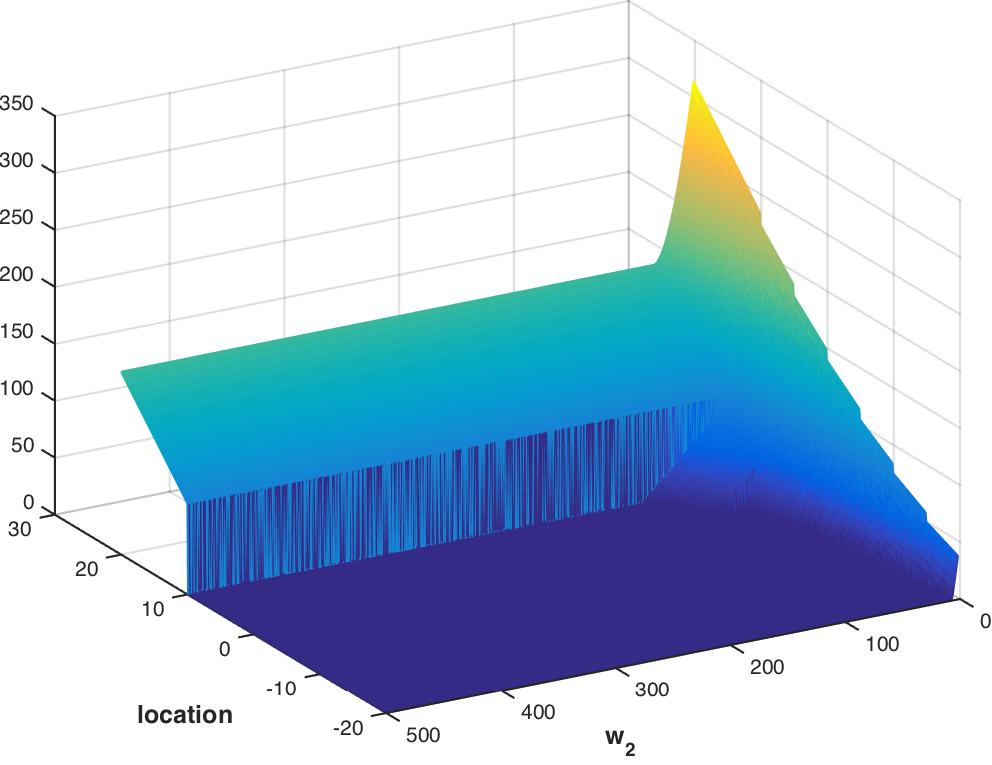
\includegraphics[width=0.8\linewidth, height=0.55\linewidth]{images/robot1d}
    \caption{The optimal value function for the multi-objective navigation domain. At low values of {\footnotesize $w_2$} the vehicle is willing to incur the movement cost to reach regions with higher linear reward.}
    \label{fig:vehicle1d}            
\end{figure}
%------------------------------------------------------------------------------

\subsection{Influenza Public Health Policy}
\label{sec:results_influenza}

Influenza viruses continuously challenge human hosts with new variants and cause complex epidemics. Compartmental models are widely used within epidemiology to investigate the spread of infection diseases such as Influenza. In this domain we investigate the efficacy of the public health policy of vaccination on a model of Influenza epidemiology by varying an infection rate parameter.

%The common components of both models can be defined as:
%\begin{itemize}
%    \item {\footnotesize $ \Action \in \left\lbrace 0, 0.25, 0.50, 1.0 \right\rbrace $} is the proportion to vaccinate 
%    \item {\footnotesize $ \Reward\left(\vec{w}, cost_{\mathtt{inf}}, cost_{\mathtt{vaccine}}, s, i, a \right) = w_1 \cdot \Reward_{\mathtt{inf}} + w_2 \cdot \Reward_{\mathtt{vaccine}}$} where, \\
%    {\footnotesize 
%        \abovedisplayskip=10pt
%        \belowdisplayskip=0pt
%        \renewcommand{\arraystretch}{1.5}
%        \begin{tabular}{ll}    
%            $ \Reward_{\mathtt{inf}}(i, cost_{\mathtt{inf}}) = $ &  $ $ \\
%            \qquad $ \begin{cases}
%            (i \geq 0) : & -cost_{\mathtt{inf}} \cdot i \\
%            \text{otherwise} : & 0 \\
%            \end{cases} $ & $ $ \\
%            $ \Reward_{\mathtt{vaccine}}(s, a, cost_{\mathtt{vaccine}}) = $ &  $ $ \\
%            \qquad $ \begin{cases}
%            (s \geq 0) : & -cost_{\mathtt{vaccine}} \cdot s \cdot a \\
%            \text{otherwise} : & 0 \\
%            \end{cases} $ & $ $ \\
%        \end{tabular}
%    } \\
%{\footnotesize $ cost_{\mathtt{inf}} $} is the incident cost of infection, akin to a burden of disease, and {\footnotesize $ cost_{\mathtt{vaccine}} $} is the unit cost of vaccination. \\    
%\end{itemize}

%\subsubsection{S-I Model}
%\label{sec:results_influenza_sd}
%
%A simple two compartment S-I epidemiological model is shown in Figure~\ref{fig:si_spec}.
%%------------------------------------------------------------------------------
%% Figure
%\begin{figure}[h!]
%    \centering
%    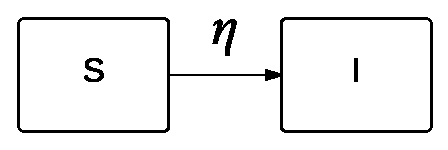
\includegraphics[width=0.3\linewidth, height=0.11\linewidth]{images/si}
%    \caption{An S-I model of Influenza epidemiology. {\footnotesize $ S $} and {\footnotesize $ I $} refer to the size of the susceptible and infected sub-populations, respectively. The infection rate is specified by {\footnotesize $ \eta$}. }
%    \label{fig:si_spec}            
%\end{figure}
%%------------------------------------------------------------------------------
%The S-I model can be formulated as a PHMDP as follows:
%\begin{itemize}
%    \item {\footnotesize $ \State = \left\langle s, i \right\rangle$}, where $ s $ and $ i $ are as defined above
%    \item The transition function {\footnotesize \Transition} for each state variable in {\footnotesize \State} is given by:    \\
%    {\footnotesize 
%        \abovedisplayskip=5pt
%        \belowdisplayskip=0pt
%        \renewcommand{\arraystretch}{1.5}
%        \begin{tabular}{ll}
%            $ \Transition\left( s' | s, i, a \right) =$ & $ \delta \left[ s' - (s - s \cdot (\eta + a)) \right] $ \\
%            $ \Transition\left( i' | s, i, a \right) =$ & $ \delta \left[ i' - (i + \eta \cdot s) \right] $ \\
%        \end{tabular}
%    }%
%    \item {\footnotesize $ \Action \in \left\lbrace 0, 0.25, 0.50, 1.0 \right\rbrace $} is the proportion of $ s $ to vaccinate 
%    \item {\footnotesize $ \Reward\left(\vec{w}, cost_{\mathtt{inf}}, cost_{\mathtt{vaccine}}, s, i, a \right) = w_1 \cdot \Reward_{\mathtt{inf}} + w_2 \cdot \Reward_{\mathtt{vaccine}}$} where, \\
%    {\footnotesize 
%        \abovedisplayskip=10pt
%        \belowdisplayskip=0pt
%        \renewcommand{\arraystretch}{1.5}
%        \begin{tabular}{ll}    
%            $ \Reward_{\mathtt{inf}}(i, cost_{\mathtt{inf}}) = $ &  $ $ \\
%            \qquad $ \begin{cases}
%            (i \geq 0) : & -cost_{\mathtt{inf}} \cdot i \\
%            \text{otherwise} : & 0 \\
%            \end{cases} $ & $ $ \\
%            $ \Reward_{\mathtt{vaccine}}(s, a, cost_{\mathtt{vaccine}}) = $ &  $ $ \\
%            \qquad $ \begin{cases}
%            (s \geq 0) : & -cost_{\mathtt{vaccine}} \cdot s \cdot a \\
%            \text{otherwise} : & 0 \\
%            \end{cases} $ & $ $ \\
%        \end{tabular}
%    } \\
%    {\footnotesize $ cost_{\mathtt{inf}} $} is the incident cost of infection, akin to a burden of disease, and {\footnotesize $ cost_{\mathtt{vaccine}} $} is the unit cost of vaccination.
%\end{itemize} 

%\subsubsection{S-I-R-S Model}
%\label{sec:results_influenza_sirs}

Influenza epidemiology is commonly investigated via a three compartment S-I-R-S model shown in Figure~\ref{fig:sirs_spec}.
%------------------------------------------------------------------------------
% Figure
\begin{figure}[h!]
    \centering
    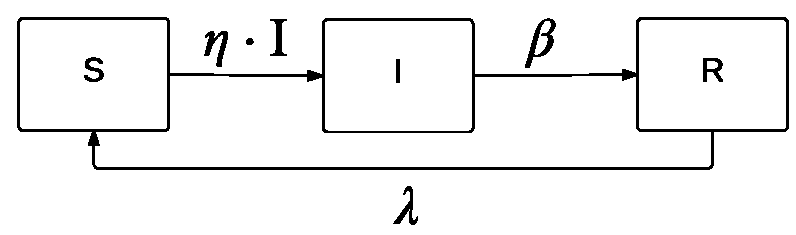
\includegraphics[width=0.5\linewidth, height=0.16\linewidth]{images/sirs}
    \caption{An S-I-R-S model of Influenza epidemiology.  {\footnotesize $ S $}, {\footnotesize $ I $} and {\footnotesize $ R $} refer to the size of the susceptible, infected and recovered sub-populations, respectively. The infection rate is specified by {\footnotesize $ \eta$}, {\footnotesize $\beta$} is the rate of recovery and {\footnotesize $\lambda$} is the rate of susceptibility.}
    \label{fig:sirs_spec}            
\end{figure}
%------------------------------------------------------------------------------

The domain is specified as follows:
\begin{itemize}
    \item {\footnotesize $ \State = \left\langle s, i, r \right\rangle$}, where $ s $, $ i $, and $ r $ are as defined above
    \item The transition function {\footnotesize \Transition} for each state variable in {\footnotesize \State} is given by:    \\
    {\footnotesize 
        \abovedisplayskip=5pt
        \belowdisplayskip=0pt
        \renewcommand{\arraystretch}{1.5}
        \begin{tabular}{ll}
            $ \Transition\left( s' | s, i, r, a \right) =$ & $ \delta \left[ s' - (s - \eta \cdot s \cdot i + \lambda \cdot r -a \cdot s) \right] $ \\
            $ \Transition\left( i' | s, i, r, a \right) =$ & $ \delta \left[ i' - (i + \eta \cdot s \cdot i - \beta \cdot i) \right] $ \\
            $ \Transition\left( r' | s, i, r, a \right) =$ & $ \delta \left[ r' - (r + \beta \cdot i - \lambda \cdot r) \right] $ \\            
        \end{tabular}
    }%
    \item {\footnotesize $ \Action \in \left\lbrace 0, 0.25, 0.50, 1.0 \right\rbrace $} is the proportion of $ s $ to vaccinate 
    \item {\footnotesize $ \Reward\left(\vec{w}, cost_{\mathtt{inf}}, cost_{\mathtt{vaccine}}, s, i, a \right) = w_1 \cdot \Reward_{\mathtt{inf}} + w_2 \cdot \Reward_{\mathtt{vaccine}}$} where, \\
    {\footnotesize 
        \abovedisplayskip=10pt
        \belowdisplayskip=0pt
        \renewcommand{\arraystretch}{1.5}
        \begin{tabular}{ll}    
            $ \Reward_{\mathtt{inf}}(i, cost_{\mathtt{inf}}) = $ &  $ $ \\
            \qquad $ \begin{cases}
            (i \geq 0) : & -cost_{\mathtt{inf}} \cdot i \\
            \text{otherwise} : & 0 \\
            \end{cases} $ & $ $ \\
            $ \Reward_{\mathtt{vaccine}}(s, a, cost_{\mathtt{vaccine}}) = $ &  $ $ \\
            \qquad $ \begin{cases}
            (s \geq 0) : & -cost_{\mathtt{vaccine}} \cdot s \cdot a \\
            \text{otherwise} : & 0 \\
            \end{cases} $ & $ $ \\
        \end{tabular}
    } \\
    {\footnotesize $ cost_{\mathtt{inf}} $} is the incident cost of infection, akin to a burden of disease, and {\footnotesize $ cost_{\mathtt{vaccine}} $} is the unit cost of vaccination.    
\end{itemize} 

%The {\footnotesize $\Action$} and {\footnotesize $\Reward$} components of the S-I-R-S model are as previously defined for the S-I model.

Figures~\ref{fig:influenza_sirs_value_function} and~\ref{fig:influenza_sirs_sensitivity} show the relationship between the susceptible sub-population {\footnotesize $s$} versus the infection rate {\footnotesize $\eta$} and the change in the infection rate {\footnotesize $\eta$} i.e. the sensitivity, respectively. The parameters of the model were set to {\footnotesize$ \beta = 0.27, \lambda = 0.23, cost_{\mathtt{inf}} = 95.0$} and {\footnotesize$cost_{\mathtt{vaccine}} = 33.0$}. In Figure~\ref{fig:influenza_sirs_value_function} we observe that the deleterious effect of low {\footnotesize $\eta$} are largely counteracted by the effect of {\footnotesize $ \lambda $}, the rate of susceptibility. For high values of {\footnotesize $s$}, a large {\footnotesize $\eta$} leads to a dramatic and rapid decline in value. Figure~\ref{fig:influenza_sirs_sensitivity} shows that the S-I-R-S model is highly sensitive to changes in the infection rate parameter {\footnotesize $\eta$}.
% and that small changes to {\footnotesize $\eta$} can lead to large changes in the parametric value function in Equation~\eqref{eq:vi_sdp_vfunc}.
%------------------------------------------------------------------------------
% Figure
\begin{figure}[h!]
    \centering
%    \begin{subfigure}[b]{0.5\textwidth}    
%        \centering
%        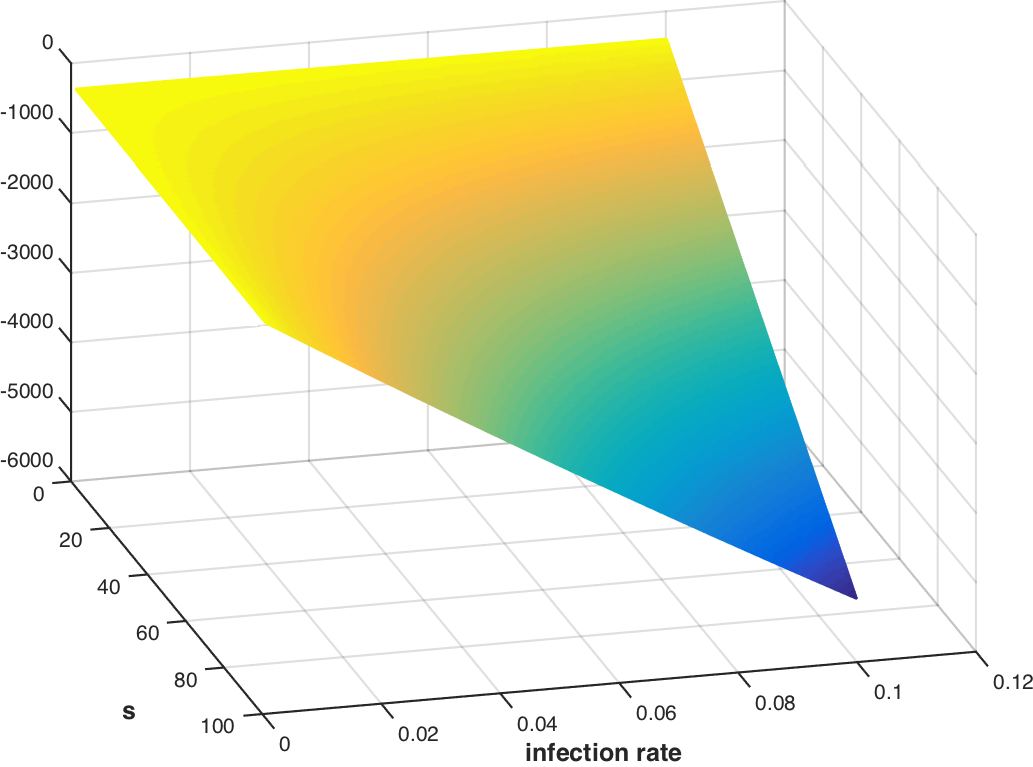
\includegraphics[width=0.8\linewidth, height=0.55\linewidth]{images/sd_infection_s}
%        \caption{S-I model.}
%        \label{fig:influenza_sd_value_function}
%        \vspace{1em}
%    \end{subfigure}  
    \begin{subfigure}[b]{0.5\textwidth}    
        \centering
        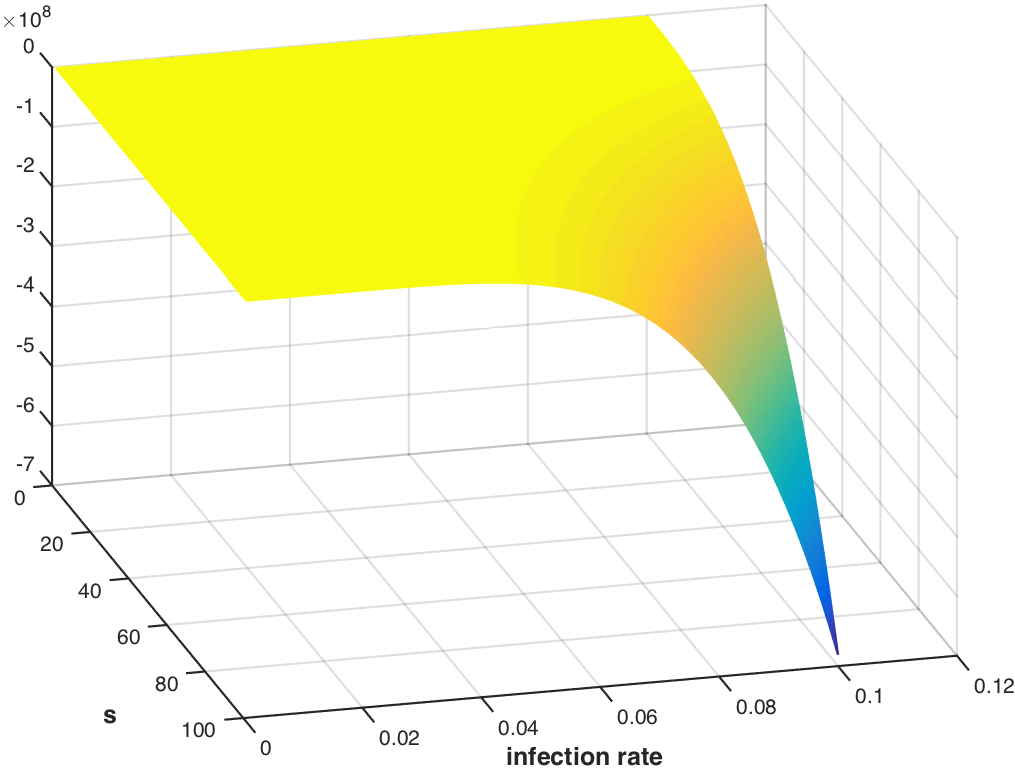
\includegraphics[width=0.8\linewidth, height=0.5\linewidth]{images/sir_infection_s}
        \caption{Susceptible vs. {\footnotesize $ \eta $}}
        \label{fig:influenza_sirs_value_function}
        \vspace{1em}
       \end{subfigure}         
    \begin{subfigure}[b]{0.5\textwidth}    
        \centering
        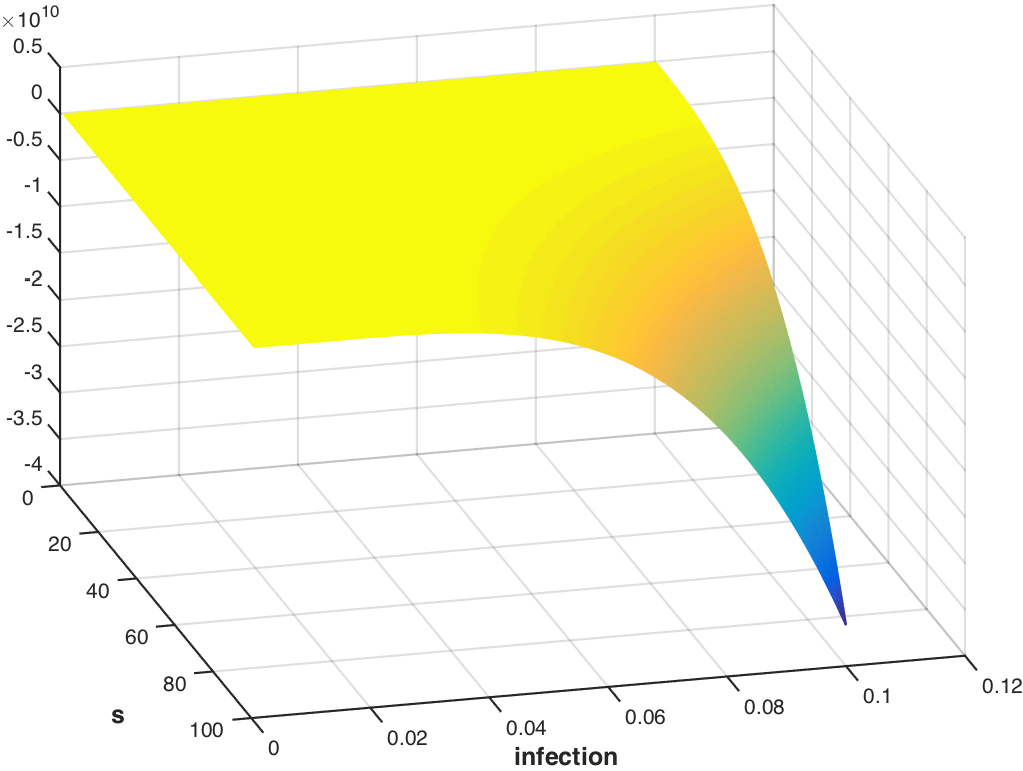
\includegraphics[width=0.8\linewidth, height=0.5\linewidth]{images/sir_infection_sensitivity}
        \caption{Susceptible vs. {\footnotesize $ \nabla \eta $} }
        \label{fig:influenza_sirs_sensitivity}
     \end{subfigure}         
    \caption{The effect of the infection rate {\footnotesize $\eta$} on the susceptible sub-population {\footnotesize $s$} under the S-I-R-S Influenza model. The S-I-R-S model is highly sensitive to higher values of {\footnotesize $\eta$}.}
    \label{fig:influenza_value_function}    
\end{figure}
%------------------------------------------------------------------------------

%------------------------------------------------------------------------------
%% Figure
%\begin{figure}[t!]
%    \centering
%    \begin{subfigure}[b]{0.5\textwidth}    
%        \centering
%        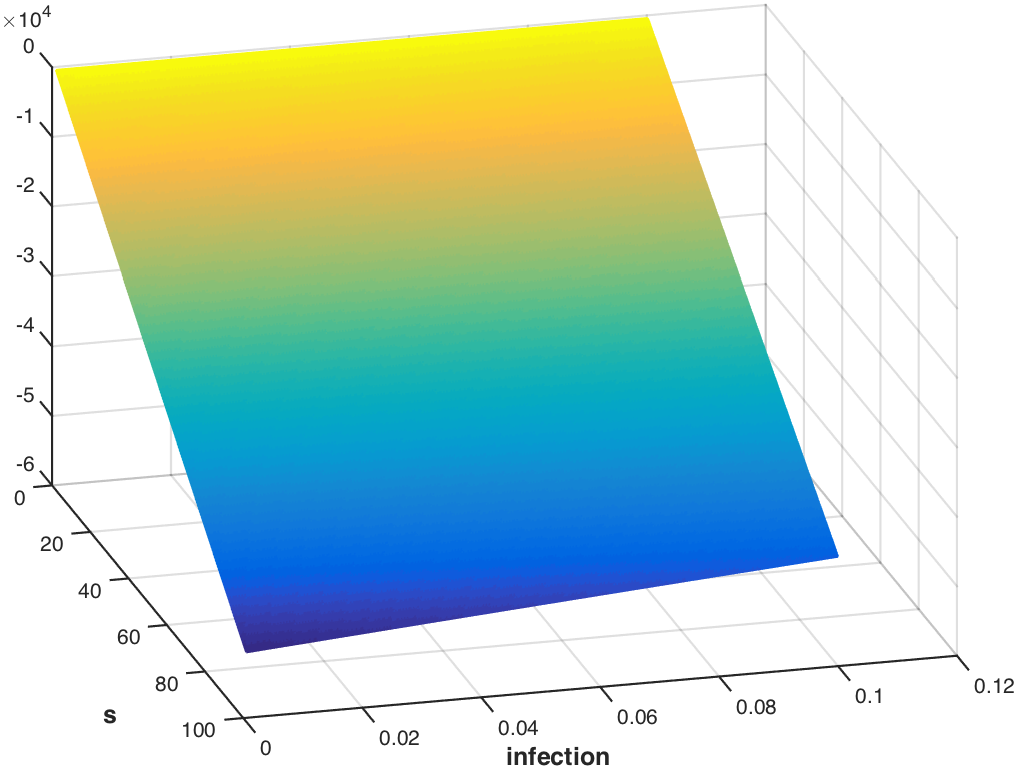
\includegraphics[width=0.8\linewidth, height=0.55\linewidth]{images/sd_infection_sensitivity}
%        \caption{S-I model.}
%        \label{fig:influenza_sd_sensitivity}
%    \end{subfigure}  
%    \begin{subfigure}[b]{0.5\textwidth}    
%        \centering
%        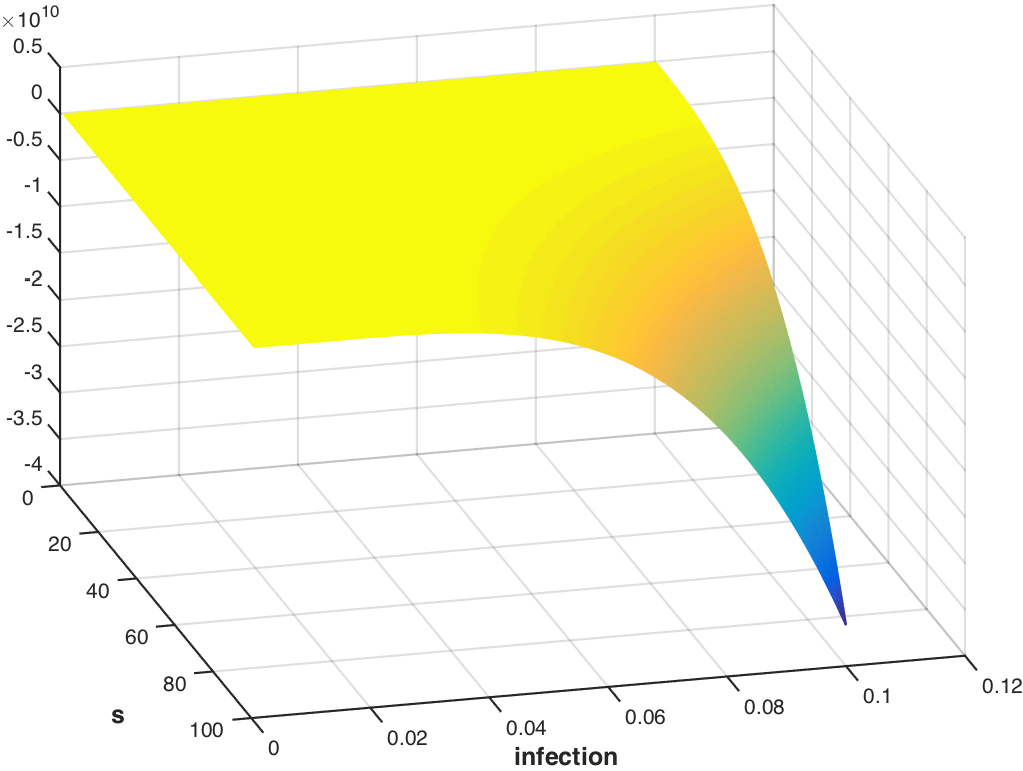
\includegraphics[width=0.8\linewidth, height=0.55\linewidth]{images/sir_infection_sensitivity}
%        \caption{S-I-R-S model.}
%        \label{fig:influenza_sirs_sensitivity}
%    \end{subfigure}  
%    \caption{The sensitivity of susceptible sub-population {\footnotesize $s$} to changes in the infection rate {\footnotesize $\eta$} under different Influenza model specifications. The S-I-R-S model is more sensitive to higher values of {\footnotesize $\eta$} than the S-I model. }
%    \label{fig:influenza_sensitivity}      
%\end{figure}
%------------------------------------------------------------------------------

\subsection{Optimal Execution}
\label{sec:results_oe}

Institutional investors often need to acquire or liquidate a number of shares within a given period of time. Indirect transaction costs are an important consideration for institutional investors who often want to transact a number of shares that exceeds the available liquidity i.e. there may not be a counterparty or counterparties that wish to take the other side of the trade at the same volume. There is a clear trade-off between the market impact of transacting immediately and the volatility of slow execution. 

In this domain we use a price impact model to investigate the optimisation of parameters within a static parameterized proportional liquidation policy, where the investor can vary the proportion of remaining inventory to sell. The domain is specified as follows:
\begin{itemize}
    \item {\footnotesize $ \State = \left\langle p, inv \right\rangle$}, where $ p $ is the price of the asset and $ inv $ is the inventory remaining
    \item {\footnotesize $ \Action \in \left\lbrace \pi\left( \theta \right) \right\rbrace$}, where {\footnotesize $ \theta \in \left( 0, 1\right)$} is the proportion of inventory to be sold
    \item The transition function {\footnotesize \Transition} for each state variable in {\footnotesize \State} is given by:    \\
    {\footnotesize 
        \abovedisplayskip=5pt
        \belowdisplayskip=0pt
        \renewcommand{\arraystretch}{1.5}
        \begin{tabular}{ll}
            $\Transition\left( p' | p, inv, \pi\left( \theta \right) \right) = $ & $\delta \left[ p' - (p + \kappa + \epsilon) \right] $ \\
            $\Transition\left( inv' | p, inv, \pi\left( \theta \right) \right) = $ & $\delta \left[ inv' - (inv - inv \cdot \pi\left( \theta \right)) \right] $ \\
        \end{tabular}
    }%
    {\footnotesize where $ \kappa $ and $ \epsilon$ are drift and discrete noise parameters, respectively.}
    \item {\footnotesize $ \Reward\left(p, p_0, inv, \pi\left( \theta \right) \right) = inv \cdot \left(\pi\left( \theta \right) \cdot p - p_0\right)$ }  
\end{itemize}

The investor aims to minimise \textit{price slippage}, which is defined as the difference between the theoretical benchmark price, {\footnotesize $p_0$}, and the actual price received.

Figure~\ref{fig:opt_execution} displays the optimal {\footnotesize$ \Horizon = 5 $} value function under the parameterized proportional liquidation policy. The parameters of the models were set to {\footnotesize$ \kappa = 1.65 \times 10^{-3}, p_0 = 10.0, p = 20.0$} and {\footnotesize $inv = \left\lbrace 0.0, 200.0\right\rbrace$}. It is clearly evident that the value function is maximised when the proportion sold, {\footnotesize $\pi\left( \theta \right) = 1.0$}, for all inventory settings. At this value of the parameter the investor maximises return by limiting exposure to price slippage.

%------------------------------------------------------------------------------
% Figure
\begin{figure}[h!]
    \centering
    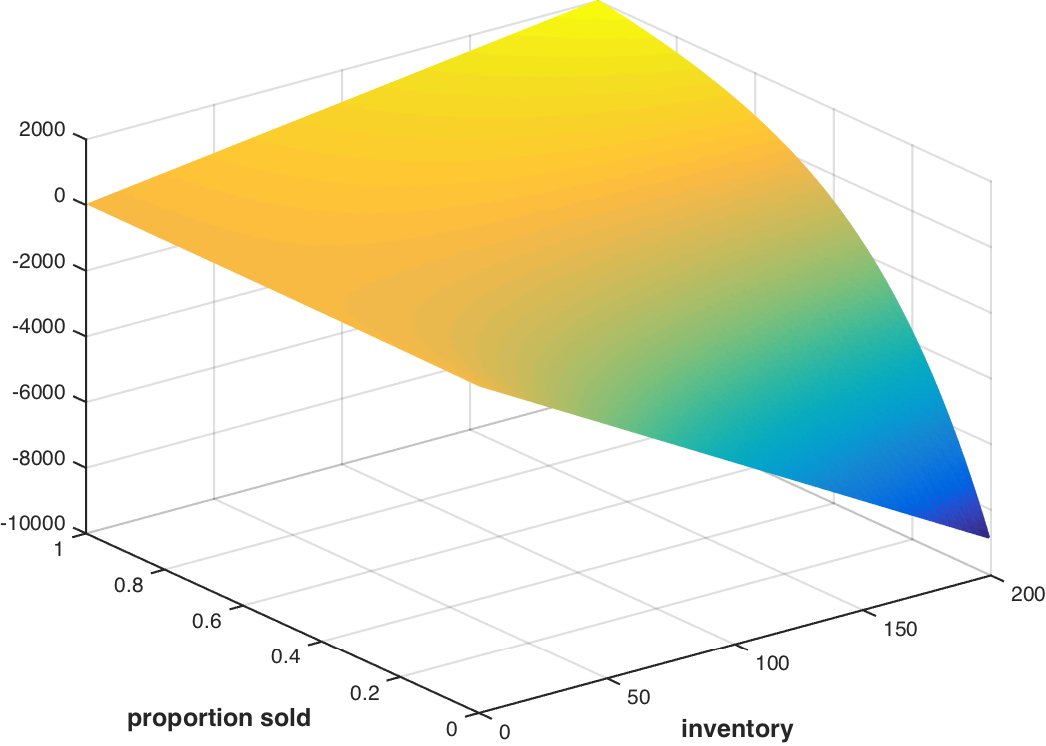
\includegraphics[width=0.8\linewidth, height=0.5\linewidth]{images/opt_execution_fraction}
    \caption{The optimal execution value function under the parameterized proportional liquidation policy. The reward obtained is maximised by increasing the policy parameter ({\footnotesize $\theta $}, the proportion sold) over all levels of inventory.}
    \label{fig:opt_execution}            
\end{figure}
%------------------------------------------------------------------------------
    \section{Conclusions and Future Work}
\label{sec:conclusion}

In this paper we introduced parameterized hybrid MDPs as a unifying framework which enables the investigation of trade-offs between multi-objective reward criteria, the examination of parameter sensitivity and the non-convex optimization of continuous policy parameters. 
We have also presented a novel parametric extension of symbolic dynamic programming that be can be used to calculate exact solutions for domains modeled within this framework. The framework and algorithm were used to calculate the first known exact and closed-form solutions to sensitivity analysis of public health policies in epidemic models and the optimization of continuous non-convex policy parameters within the optimal execution problem in finance.

There are a number of avenues for future research. Firstly, it is important to examine more general representations of the reward and transition functions while still guaranteeing exact solutions. Another direction of research lies within improving the scalability of the algorithm by either extending techniques for Algebraic Decision Diagrams~\parencite{Bahar_JoFMiSD_1993} from APRICODD~\parencite{St-Aubin_NIPS_2000} under the current restrictions on the reward and transition functions, bounded error compression for 
XADDs~\parencite{Vianna_UAI_2013} for more expressive representations, or lazy approximation of value functions as piecewise linear XADDs~\parencite{Li_AAAI_2005}. The advances made within this paper open up a number of potential novel research paths which may be used to progress solutions to multi-objective MDPs, sensitivity analysis and optimization of policy parameters.

%--------------------------------------------------------------------------------------------------
% Bibliography
%--------------------------------------------------------------------------------------------------
\newpage
{\small
\printbibliography
}
\end{document}